\documentclass[10pt,twocolumn,letterpaper]{article}

\usepackage{wacv}
\usepackage{times}
\usepackage{epsfig}
\usepackage{graphicx}
\usepackage{amsmath}
\usepackage{amssymb}

% Include other packages here, before hyperref.
\usepackage{sidecap}
\usepackage{enumerate}

% If you comment hyperref and then uncomment it, you should delete
% egpaper.aux before re-running latex.  (Or just hit 'q' on the first latex
% run, let it finish, and you should be clear).
%\usepackage[pagebackref=true,breaklinks=true,letterpaper=true,colorlinks,bookmarks=false]{hyperref}

%\wacvfinalcopy % *** Uncomment this line for the final submission

\def\wacvPaperID{****} % *** Enter the wacv Paper ID here
\def\httilde{\mbox{\tt\raisebox{-.5ex}{\symbol{126}}}}

% Pages are numbered in submission mode, and unnumbered in camera-ready
\ifwacvfinal\pagestyle{empty}\fi
\setcounter{page}{1}
\begin{document}

%%%%%%%%% TITLE
\title{The usefulness of image super-resolution for other vision tasks}

% Authors at the same institution
\author{Yujian Wang \hspace{2cm} Dengxin Dai \\
ETH Zurich\\
{\tt\small yjwang@student.ethz.ch}
}
% Authors at different institutions
% \author{First Author \\
% Institution1\\
% {\tt\small firstauthor@i1.org}
% \and
% Second Author \\
% Institution2\\
% {\tt\small secondauthor@i2.org}
% }

\maketitle
\ifwacvfinal\thispagestyle{empty}\fi

%%%%%%%%% ABSTRACT
\begin{abstract}
Despite the great advances made on image super-resolution (ISR)
  during the last years, its performance has solely been evaluated
  perceptually. Thus, it is still unclear whether ISR systems are
  useful for other vision tasks in practice. In this paper, we present
  the first comprehensive study and analysis of ISR for other vision
  applications. In particular, five state-of-the-art ISR methods are
  evaluated on five popular vision tasks, namely edge detection, image
  segmentation, semantic labeling, digit recognition, and face
  recognition. We show that ISR, in addition to improving the
  perceptual quality of images, does improve the performance of other
  vision tasks when the input images are of relatively
  `low-resolution'. We also demonstrate that the standard perceptual
  evaluation criteria, such as PSNR, correlate well the the usefulness
  of ISR methods to other vision tasks. We hope this work will inspire
  the community to deploy ISR as a preprocessing component of the
  systems of other vision tasks if the input data are of relatively
  low-resolution, and to evaluate ISR methods in real vision
  applications.
\end{abstract}

%%%%%%%%% BODY TEXT

%------------------------------------------------------------------------- 
\section{Introduction}
\label{sec:intro}
Image super-resolution (ISR) aims to sharpen smooth rough edges and
enrich missing textures in images that have been enlarged using a
general up-scaling process (such as a bilinear or bicubic process),
thereby delivering an image with high-quality
resolution~\cite{Freeman-CGA-2002, Yang-TIP-2010, Zeyde-CS-2012,
  Timofte-ICCV-2013, Dong-ECCV-2014, JOR:EG15}. ISR systems can be
used to adapt images to displaying devices of different dimensions, to
map image textures to 2D/3D shapes, and to deliver pleasing
visualization for data that are inherently low-resolution such as
image or videos from surveillance cameras.  Despite the popularity of
ISR in the past years, their performance has merely been evaluated
perceptually and/or by evaluation criteria reflecting perceptual
quality such as PSNR and SSIM. Therefore, it is still unclear whether
ISR is useful in general for other vision tasks and whether the
perceptual criteria also reflect the usefulness of the ISR methods for
other vision tasks. This paper addresses the problems.

% Although ISR has been raising more attention, its potential usefulness
% for other popular vision tasks is largely ignored, so does the
% evaluation of ISR in such a way.
We here present reasons why ISR can be useful for other vision tasks, in
addition to improving perceptual quality. As we know, most of current
vision systems consist in two phases: training and testing. Although
features have been designed to overcome the influence of scale
changes, it is still helpful 1) to keep training and testing images
being of the same/similar resolution, and 2) to convert input images to the resolution for which the features and the models
are designed, if they are of very different resolution.  It happens quite common that training and
testing data are of different resolutions, \eg training images are
from expensive sensors while testing images from cheap ones. If
testing images are of higher resolution, downsampling them
with linear filters does the job. If the opposite
holds, however, sophisticated ISR methods
are required to super-resolve the testing images. Also, most vision systems are designed and optimized
(\eg the features) for images of the most `popular' resolution at the
time. ISR is useful to super-resolve images which are of
lower-resolution than the images for which the features and models are designed and learned. One example is object recognition with surveillance cameras where popular features
for object detection are designed for normal images which are of
higher-resolution than surveillance scenes in general. For this case, even the
training data and the testing data are of the same resolution, ISR is
still helpful to super-resolve all the data so that
the features can be computed at the appropriate resolution. 

% Although image
% features are often designed to overcome the influence of scale
% changes, we found in the experiments that performing ISR does improve
% the performance of other vision tasks.

In order to sufficiently sample the space of ISR methods and potential
vision tasks, five ISR methods are chosen and evaluated on four popular
vision applications. The ISR methods are Zeyde
\etal~\cite{Zeyde-CS-2012}, ANR~\cite{Timofte-ICCV-2013},
A+~\cite{Timofte-ACCV-2014}, SRCNN~\cite{Dong-ECCV-2014}, and
JOR~\cite{JOR:EG15}. 
% They are chosen due to the wide coverage from
% very basic methods to the state-of-the-arts. 
The four vision
applications include image boundary detection, image labeling, digit recognition, and face detection. The tasks are chosen 
because they are representatives of current low- and high-level vision
tasks. The data of digits and faces are chosen because low-resolution
inputs are very likely to occur in these two fields. For all the
tasks, we use standard methods and standard datasets, while changing
the modes of the input images: from downsampled low-resolution images,
to super-resolved images by different ISR methods, and to the original
images. The experimental results suggest that ISR is generally useful
for practical vision tasks if the resolution of the input images are
low, and that the standard evaluation criterion PSNR of ISR correlate quite
well with the usefulness of ISR methods for other vision tasks, but
cannot measure it accurately. 

% The paper is organized as follows. Section~\ref{sec:relatedwork}
% reports relevant work. Evaluation on the four vision tasks are
% conducted in Section~\ref{sec:ed} to Section~\ref{sec:fr}. Finally,
% the paper concludes in Section~\ref{sec:conclusion}.

\section{Related Work}
\label{sec:relatedwork}
There is a large body of work addressing image super-resolution
task. We breifly summarize them. % They can be roughly classified into two groups: single image
% super-resolution (SISR) and multiple image ISR (MISR). As the names
% suggest, SISR works with a single low-resolution (LR) image as input,
% while MISR works with multiple LR images (\eg from different views) as
% inputs. Since MISR are more restricted, this paper focuses on SISR.
% We will briefly overview some of the main research directions of SISR.
The oldest direction is represented by variants of interpolation, such as Bilinear and Bicubic~\cite{Duchon-JAM-1979,Thevenaz-BOOK-2000}. They
represent the simplest and the most popular methods. However, they
often produce visual artifacts such as blurring, ringing, and
blocking, which follows the fact that their assumptions of smoothness
and band-limited image data handly hold in real cases. Due to these
reasons, more realistic priors and regularizations have been
developed, such as the sparse derivative priors
in~\cite{Tappen-WSCTV-2003}, the PDE-based regularization
in~\cite{Tschumperle-PAMI-2005}, and the edge smoothness prior
in~\cite{Dai-CVPR-2007}. Despite the improvement by these methods, the
explicit forms of priors are still insufficient to express the
richness of real-world image data.

In recent years, example-based image super-resolution has raised the
most attention due to its good performance and simplicity. For this
stream, the task is to upsample an image, given the low-resolution
(LR) image and a collection of pairs of LR images and their
corresponding high-resolution (HR) images. The pioneering
work~\cite{Freeman-CGA-2002} transfers the HR patches of the most
similar LR patches directly and regularizes the solution by MRF. The
idea has been extended in a variety of ways: \cite{Chang-CVPR-2004}
employs Embedding technique for the regularization; \cite{JOR:EG15}
jointly learns a collection of local regression functions and
adaptively selects the most suitable ones for test patches.
\cite{Yang-TIP-2010} learns coupled dictionaries for LR and HR patches
via forcing shared encoding; \cite{Timofte-ICCV-2013,
  Timofte-ACCV-2014} combine the two ideas for efficient systems by
learning local regression functions for the atoms of the
dictionary. The exception is the work SRCNN~\cite{Dong-ECCV-2014}
which learns the transformation from LR images to their HR version via
convolutional neural network. Since example-based methods obtain
state-of-the-art performance for ISR, our evaluation is focused
mostly on this stream, with an comparison to Bicubic Interpolation.

The work most relevant to ours is~\cite{SR:benchmark}, where different
ISR methods are evaluated. While sharing similarities, the two methods
still differs significantly. \cite{SR:benchmark} conducted user
studies for perceptual evaluation, solely with visual comparison and
under evaluation criteria such as PSNR. Our work, however, integrates
ISR methods into systems of other practical vision applications and
evaluates the usefulness of ISR to these vision tasks. There are also works~\cite{face:SRTIP, face:SR08} proving that face super-resolution is useful for face recognition. However, they focus merely on faces and the super-resolution methods specific to faces. Our work, however, evaluates general ISR methods with a variety of popular vision tasks. 



\section{Evaluation}
\label{se:evalucation}

In this section, we briefly describe the five ISR methods:  Zeyde \etal~\cite{Zeyde-CS-2012},
ANR~\cite{Timofte-ICCV-2013}, A+~\cite{Timofte-ACCV-2014},
SRCNN~\cite{Dong-ECCV-2014}, and JOR~\cite{JOR:EG15}, followed by the
evaluation on the four vision tasks. 
 The five methods, starting with the results of Bicubic npterpolation,  learn from examples to recover the missing high-frequency parts. As to the examples, the five methods are all trained with the same training dataset
from~\cite{Yang-TIP-2010}, which consists of $91$ images. For
implementation, we use the codes from the authors directly. Readers
are referred to the papers for corresponding details. As to scaling
factors, we evaluate with $\times$3 and $\times$4.


For datasets, we use the standard ones for the tasks. To generate inputs
for our evaluation, we downscale the original images from the datasets
by factors $\times$3 and $\times$4 to create the low-resolution (LR)
images and then upscale them by each of the five ISR methods to the resolution of the original images, which are then used as the inputs for the vision tasks. 
The standard approaches to the four tasks are
then applied to all super-resolved versions of the images, once for each version. The corresponding performances are recorded to evaluate the usefulness of ISR methods for the vision tasks, with a comparison to Bicubic Interpolation.


%simple interpolation is more pronounced with large scaling factor.
% We follow the data representation and the general framework
% from . The basic idea is that the low frequency
% part can be approximated reasonably well by a
% fast interpolation kernel such as bicubic, thus the problem
% reduces to the estimation of the fine details. It has also
% been found that gradient features are most relevant to high resolution
% details. Therefore, the LR and HR patches are represented
% as follows. In the training, the HR images are downscaled
% to the LR corresponding images for a given upscaling
% factor. Then, the LR image is bicubically interpolated by the
% same factor to get to an interpolated HR image. The first and
% second order gradient filters are applied vertically and horizontally
% to this image, and the LR image patches x are represented
% as the concatenation of corresponding gradient responses.
% Note that the interpolated HR images are also called
% LR images, as the high-frequency details are still missing.


\subsection{Boundary Detection}
\label{sec:ed}



Boundary Detection (BD) is a very popular low-level vision
task and serves as a crucial component for many high-level vision
systems~\cite{Martin-ICCV-2001, isola2014crisp}. This section evaluates
the usefulness of ISR methods for BD.  
We use Crisp Boundary Detection~\cite{isola2014crisp} (CBD), which is an
unsupervised algorithm, deriving an affinity measure with point-wise
mutual information between pixels and utilizing this affinity with
spectral clustering method to detect boundaries. It produces
pixel-level boundaries and achieves state-of-art results.  The
performances are evaluated on the BSDS300
dataset~\cite{Martin-ICCV-2001}. The whole dataset consists of 300
images (200 for training and 100 for testing) along with human
annotations.  The quality of detected boundaries is evaluated 
by precision-recall (PR) curves, following Berkeley Benchmark~\cite{arbelaez2007berkeley}.  


\begin{table} [tb]\small{
\centering
\resizebox{0.5\textwidth}{!}
{
\begin{tabular}{|l|c|cccccc|c|}
  \hline
  \multicolumn{2}{|c|}{BSDS300} & Bicubic & Zeyde~\etal & ANR & SRCNN & A+ & JOR & Original \\
  \multicolumn{2}{|c|}{\emph{avg.}} & &\cite{Zeyde-CS-2012}& \cite{Timofte-ICCV-2013}& \cite{Dong-ECCV-2014} & \cite{Timofte-ACCV-2014} &\cite{JOR:EG15} & \\
  \hline
  \hline
  \textbf{$\times$3} & PSNR & 27.15 & 27.87 & 27.89 & \underline{28.10} & 27.84 & \textbf{28.17} & --- \\
  & SSIM & 0.736 & 0.770 & 0.773 & \underline{0.777} & 0.772 & \textbf{0.781} & --- \\
  & IFC & 2.742 & 3.202 & 3.248 & 3.131 & \underline{3.253} & \textbf{3.367} & --- \\
  & NQM & 27.42 & 31.81 & 31.96 & 31.28 & \underline{32.15} & \textbf{32.42} & --- \\
  \hline
  & AUC & 0.647 & 0.671 & 0.663 & 0.669 & \underline{0.674} & \textbf{0.675} & 0.696 \\
  \hline
  \textbf{$\times$4} & PSNR & 25.92 & 26.51 & 26.51 & 26.66 & \textbf{26.77} & \underline{26.74} & --- \\
  & SSIM & 0.667 & 0.697 & 0.699 & 0.702 & \textbf{0.709} & \underline{0.707} & --- \\
  & IFC & 1.839 & 2.196 & 2.232 & 2.118 & \textbf{2.325} & \underline{2.316} & --- \\
  & NQM & 21.15 & 24.30 & 24.38 & 24.19 & \textbf{24.98} & \underline{24.95} & --- \\
  \hline
  & AUC & 0.595 & 0.646 & 0.635 & 0.651 & \underline{0.656} & \textbf{0.657} & 0.696 \\
  \hline
\end{tabular}
}
\caption{Average PSNR values of ISR methods on BSDS300 and average AUC values of boundary detection via CBD~\cite{isola2014crisp} on the super-resolved images by the ISR methods and the original images. The best one is shown in \textbf{bold} and the second best  \underline{underlined}.}
\label{tab:ed}}
\end{table}

\begin{figure} [tb]
\centering
% \begin{tabular}{cc}
%   \hspace{-2 mm}
%   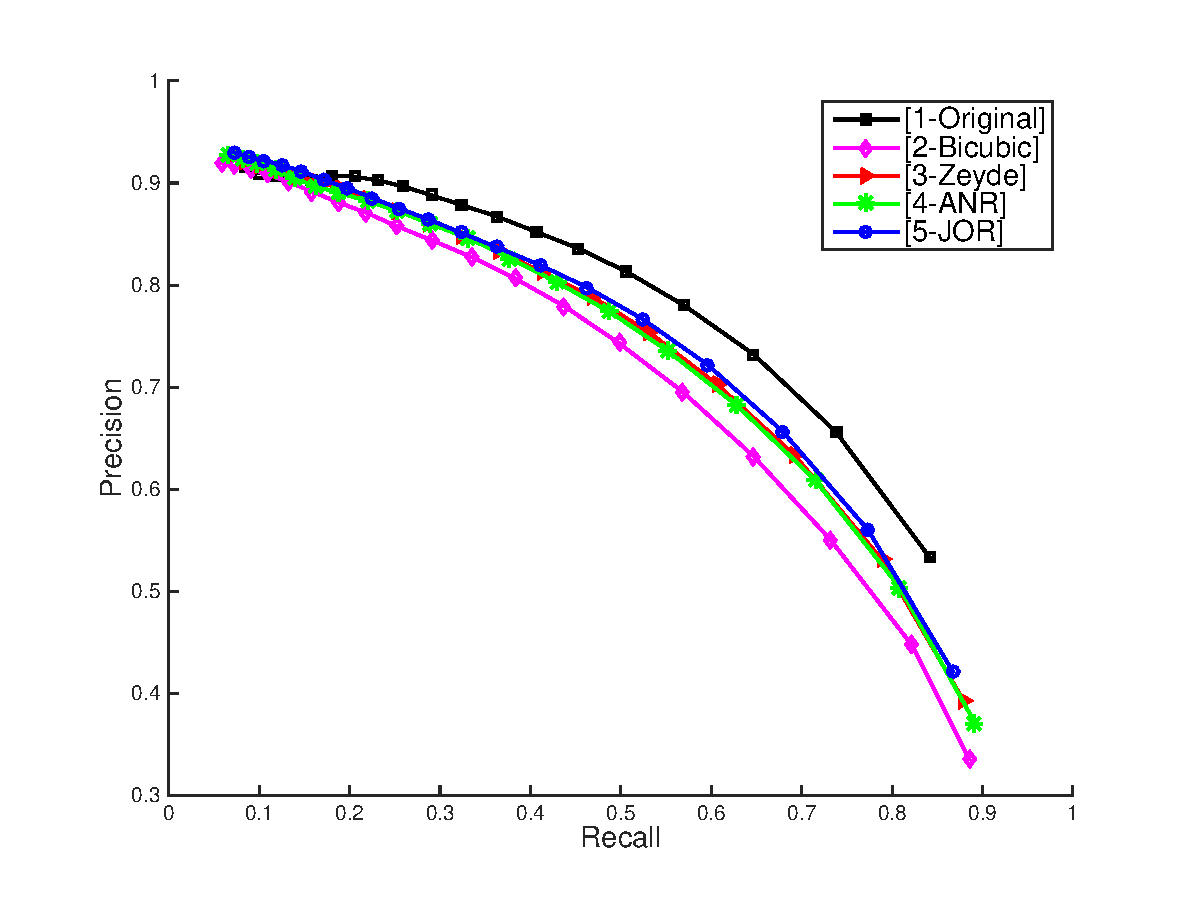
\includegraphics[width = 0.4\textwidth]{fig/pr_all_crisp_x4_zeydeanr.eps} &
%   \hspace{-4.5 mm} \\
%   \footnotesize{\text{(a) PR curves with scaling factor x4}} \\
%   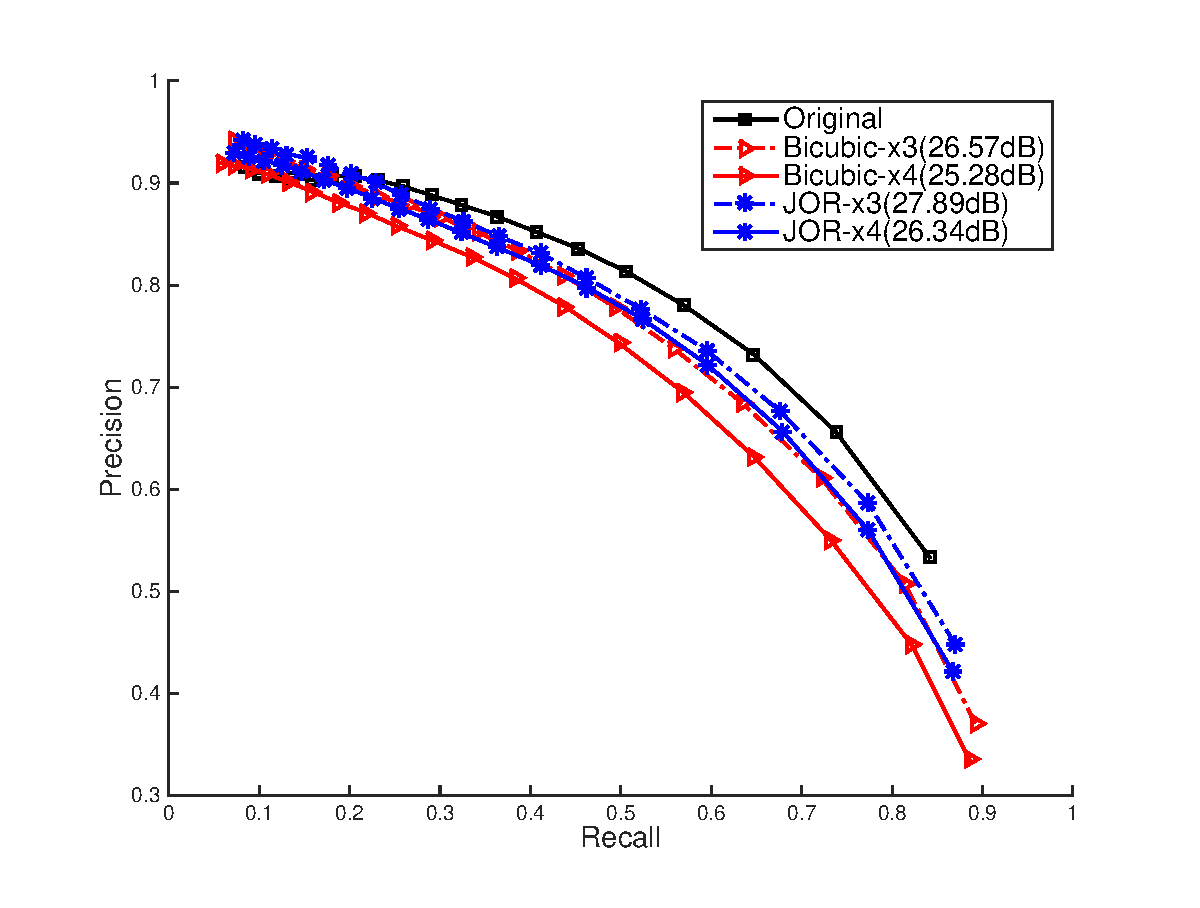
\includegraphics[width = 0.4\textwidth]{fig/pr_jor_crisp_x3x4.eps} \\
%   \footnotesize{\text{(b) PR curves with scaling factor x3 and x4}} \\
% \end{tabular}
\begin{tabular}{c}
  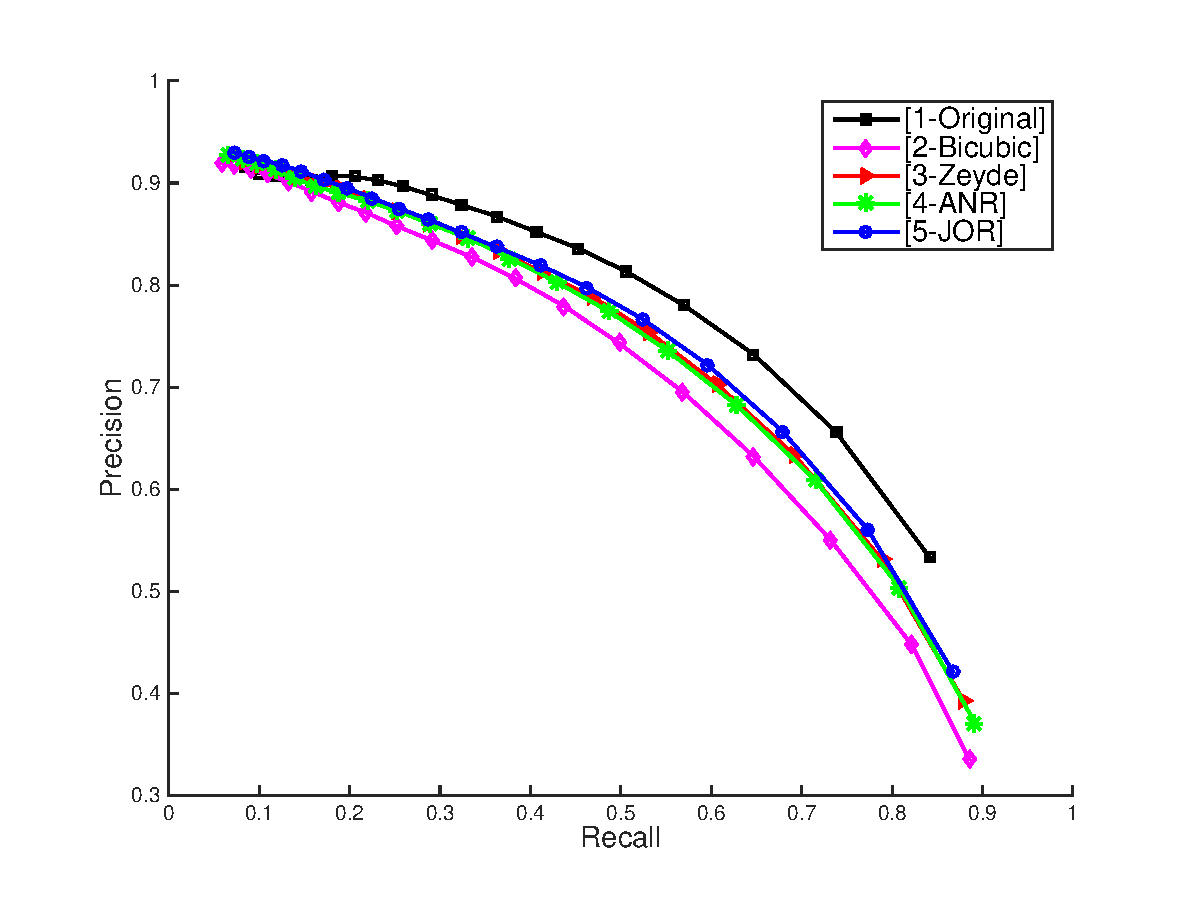
\includegraphics[width = 0.4\textwidth]{fig/pr_all_crisp_x4_zeydeanr.eps} \\
  \footnotesize{\text{(a) PR curves with scaling factor x4}} \\
  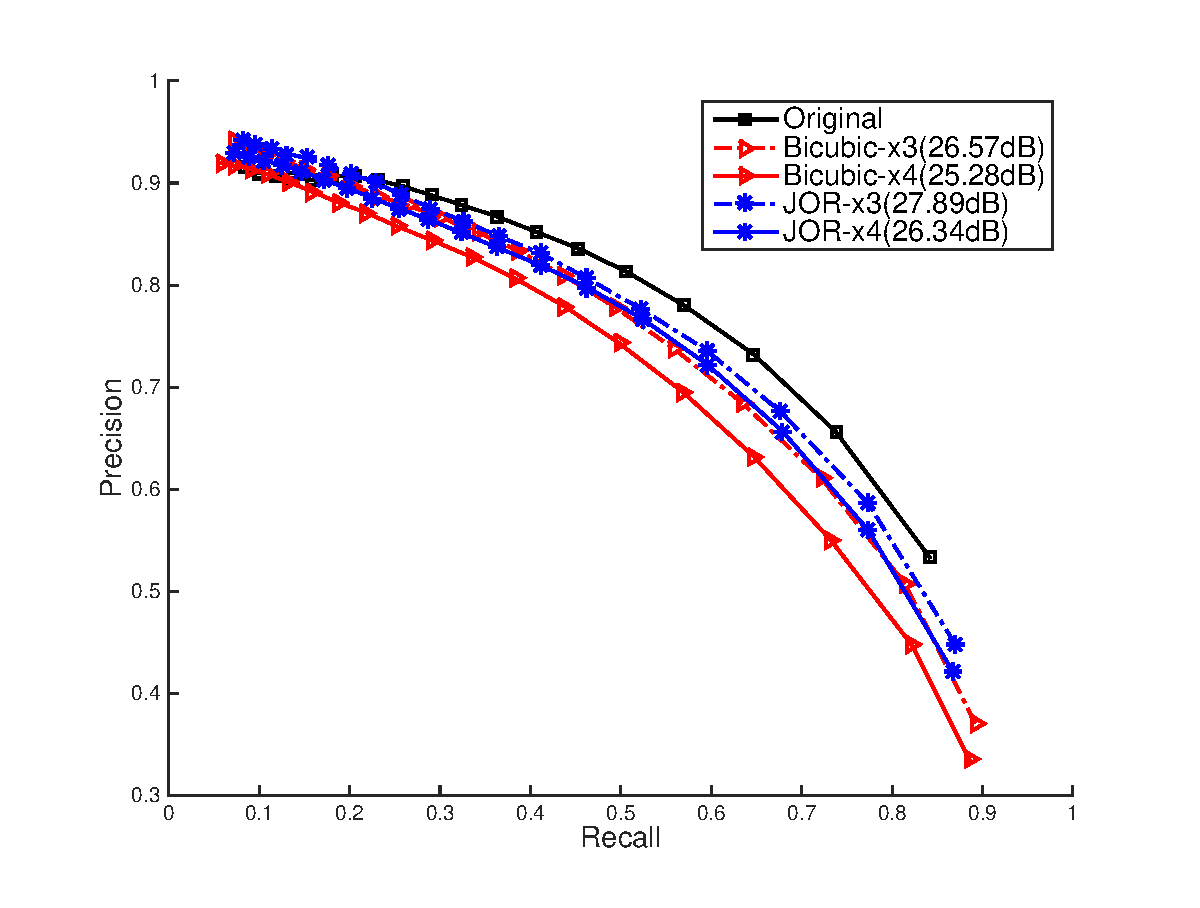
\includegraphics[width = 0.4\textwidth]{fig/pr_jor_crisp_x3x4.eps} \\
  \footnotesize{\text{(b) PR curves with scaling factor x3 and x4}}
\end{tabular}
\caption{Average PR curves of boundary detection via CBD~\cite{isola2014crisp} on the super-resolved images by some of the five ISR methods and on the original images of BSDS300.  (a) curves for scaling factor x4, where  SRCNN and A+ are not shown for visual clarity as they are very similar to JOR. (b) a comparison of scaling factor x3 and x4, where only Bicubic Interpolation and JOR are shown for visual clarity. See the text for detailed analysis.}
  \vspace{-3 mm}
\label{fig:ed_method}
\end{figure}

% Each image comes
% with at least one human-labeled boundary map and has a size of either
% 321$\times$481 or 481$\times$321 pixels.

Table~\ref{tab:ed} lists the AUC values of BD on the seven sets of images, along with the PSNR values of corresponding ISR methods, and Fig.~\ref{fig:ed_method} shows the average PR curves. From the table and the figure, it can be observed that ISR methods does improve, over simple interpolation, the performance of BD when input images are of low-resolution. This is because ISR methods perform better in increasing the resolution of the LR images to the resolution for which the BD method (CBD~\cite{isola2014crisp} in this case) was designed. CBD uses highly localized features to predict pixel-level boundaries, whose accuracy is affected largely by the recovered details locally. As a result, the five learning-based ISR methods all perform better than Bicubic Interpolation. 
This suggest that ISR should be considered as a preprocess step for image BD if the input images are of LR. One may argue that adapting the BD method may increase its performance for LR images. It is true, but we have to admit that most of the methods for high-level vision tasks are designed for images of the most popular resolution at the time. CBD is just one example. Therefore, enhancing the resolution of LR inputs is much easier than adapting all such high-level vision systems.  

It can also be found that PSNR correlates well with the usefulness of ISR methods for the task of BD. ISR methods which yield high PSNR values often also have large AUC values for BD. In general, SRCNN, A+, and JOR are the most useful ISR methods for the task of BD. However,  PSNR is not very accurate to predict the usefulness of ISR methods for BD.   
For instance, Zeyde \etal outscores ANR in terms of AUC despite of having a lower PSNR value, when factor $\times$4 is used. This suggests that measuring the usefulness of ISR methods directly for BD in a real system is necessary. 
The third finding from the table and figure is that ISR methods are more useful when the scaling factor is larger, which means they are mostly needed when the input images are of very low-resolution.  

In Fig.~\ref{fig:ed_cbd}, we show two image examples, with the super-resolution results and their corresponding BD results. From the figure, it is evident that example-based ISR methods improve the quality of BD results with sharper true boundaries and fewer spurious ones. However, there is still a large room for improvement as the OB results on the super-resolved images by the ISR methods are still substantially worse than the result on the original (`HR') image.       


% Fig.~\ref{fig:ed_method} illustrates the PR curves
% obtained by the CBD approach. Results of A+ and SRCNN are not
% drawn since they both have similar curves with the JOR method. As for
% the precision-recall curves, a curve that is farther away from the
% origin would be preferred as it indicates a higher recall or precision
% when the other value is fixed. As Figure~\ref{fig:ed_method}
% illustrates, a well designed ISR algorithm like Zeyde \etal, ANR and
% JOR could help improve the accuracy of Crisp Boundary Detection.

% It is also noticed that ISR methods above make different improvement
% in boundary detection due to different PSNR value. Here we use the area
% under precision-recall curve (AUC) as criteria to evaluate the
% accuracy of detected boundaries. As Table~\ref{tab:ed} demonstrates,
% the PSNR value correlates well with the accuracy of boundaries
% detected by CBD approach. In particular, the larger PSNR value an ISR
% method gets, the more accurate boundaries we detect in corresponding
% super-resolved dataset. One important reason is that the CBD approach
% uses highly localized features and predicts pixel-level boundaries. It
% is thus sensitive to the properties of neighboring pixels and its
% accuracy is likely to be affected by correctness of pixel
% interpolation. As a result, the five learning-based ISR methods all
% perform better than simple Bicubic interpolation. What's more, the JOR
% and A+ methods tie for the largest PSNR value among all six ISR
% methods with factor $\times$3 and $\times$4 and they also have the
% first and second highest AUC value, indicating that they both perform
% well in terms of PSNR and in real boundary detection tasks.

% However, it is important to point out that an ISR method with larger
% PSNR value is not guaranteed to perform better in real boundary detection
% as well. On one hand, we may have fluctuations in statistics such as
% Zeyde \etal outscoring ANR despite of a lower PSNR value with factor
% $\times$4. On the other hand, the AUC value may not be the perfect
% criteria as it provides little information about the shape of the
% precision-recall curve. But in general, it can be concluded that the
% PSNR value has a strong positive correlation with the accuracy of boundary
% detection.

% As for the same ISR method, altering the resizing scale of the dataset
% affects the accuracy of edges as well. It is apparent that a upscaled
% image tends to have more artifacts when increasing the resizing
% scales, resulting in a lower edge-detection accuracy. We also notice
% that a larger resizing scale tends to amplify the performance
% difference between different ISR methods, as
% Figure~\ref{fig:ed_factor} demonstrates.



% \begin{SCfigure}
%   \centering
%   \caption{Average precision-recall curves of the accuracy of edges
%     detected by the CBD method on multiple datasets. The datasets
%     include the test set of BSDS300 and four of its super-resolved
%     versions, using two ISR methods of Bicubic and JOR and scaling
%     factor of $\times$3 and $\times$4 each. Precisions and recalls are
%     averaged over all images in corresponding datasets.}
%   \includegraphics[width = 0.6\textwidth]%
%     {fig/pr_jor_crisp_x3x4.eps}% picture filename
% \label{fig:ed_factor}
% \end{SCfigure}

\begin{figure*} [tb]
\begin{tabular*}{0.5\textwidth}{ccccccc}
      (a) Original & (b) Bicubic & (c) Zeyde & (d) ANR & (e) SRCNN & (f) A+ & (g) JOR \\  
  \hspace{-2mm}
  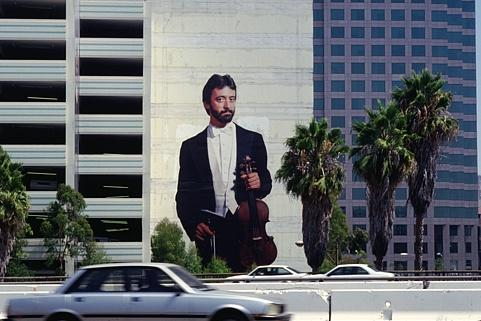
\includegraphics[width=2cm]{fig/119082_g.jpg} & \hspace{-4mm}
  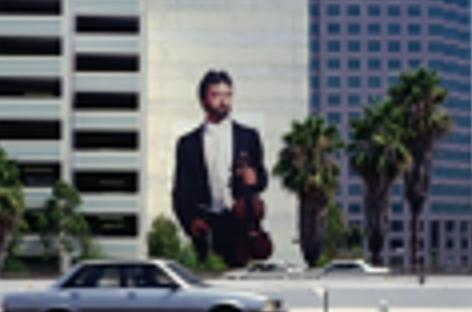
\includegraphics[width=2cm]{fig/119082[2-Bicubic]_g.jpg} & \hspace{-4mm}
  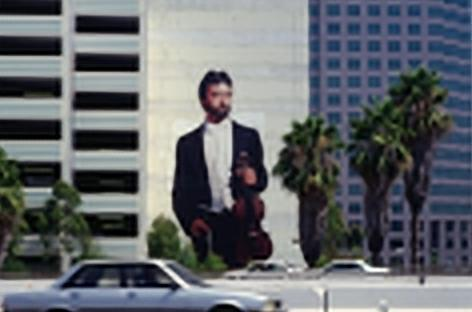
\includegraphics[width=2cm]{fig/119082[3-Zeyde]_g.jpg} & \hspace{-4mm}
  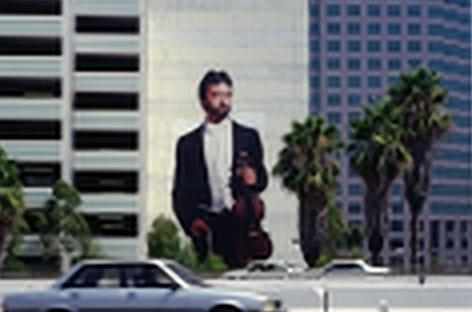
\includegraphics[width=2cm]{fig/119082[4-ANR]_g.jpg} & \hspace{-4mm}
  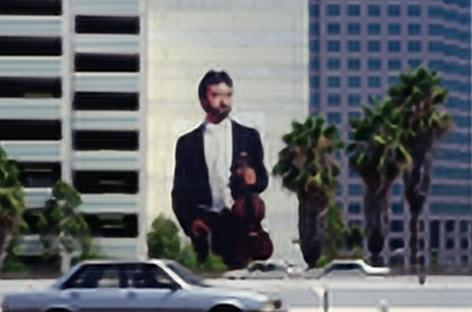
\includegraphics[width=2cm]{fig/119082[5-SRCNN]_g.jpg} & \hspace{-4mm}
  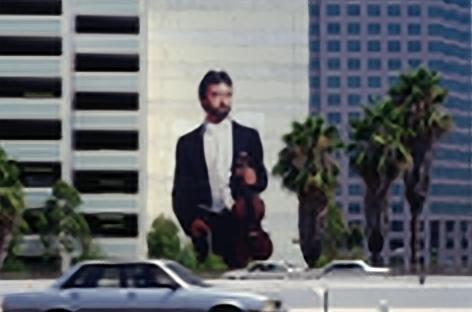
\includegraphics[width=2cm]{fig/119082[6-A+]_g.jpg} & \hspace{-4mm}
  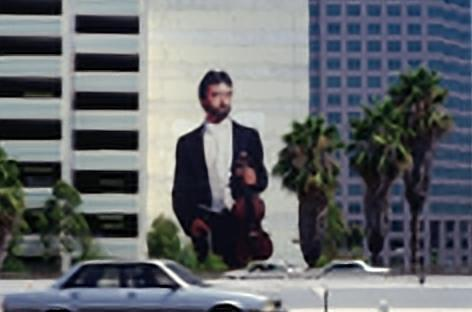
\includegraphics[width=2cm]{fig/119082[7-JOR]_g.jpg} \\
  PSNR & 22.06 & 22.83 & 22.69 & 23.13 & 23.17 & 23.14 \\     
  \hspace{-2mm}
  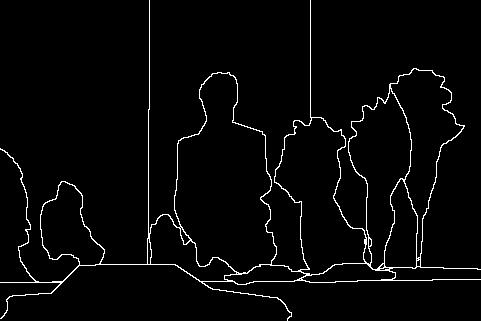
\includegraphics[width=2cm]{fig/119082_seg.jpg} & \hspace{-4mm}
  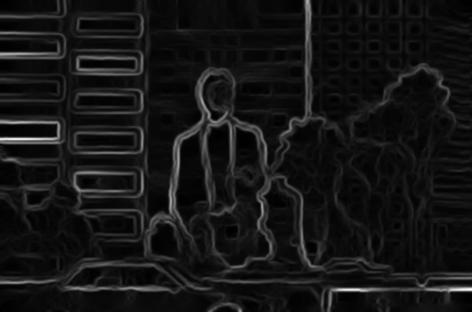
\includegraphics[width=2cm]{fig/119082[2-Bicubic]_crisp.jpg} & \hspace{-4mm}
  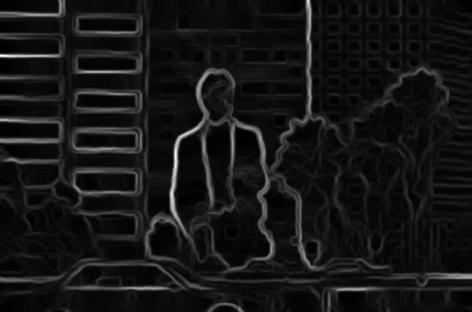
\includegraphics[width=2cm]{fig/119082[3-Zeyde]_crisp.jpg} & \hspace{-4mm}
  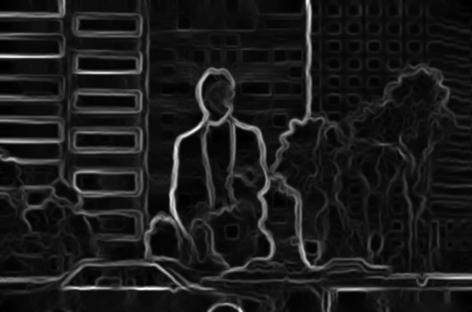
\includegraphics[width=2cm]{fig/119082[4-ANR]_crisp.jpg} & \hspace{-4mm}
  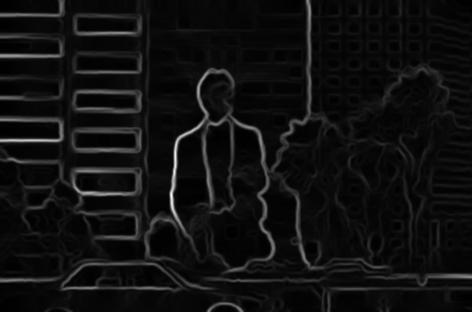
\includegraphics[width=2cm]{fig/119082[5-SRCNN]_crisp.jpg} & \hspace{-4mm}
  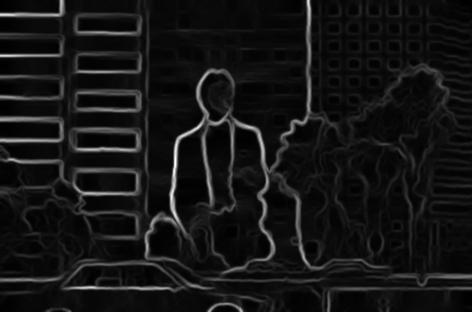
\includegraphics[width=2cm]{fig/119082[6-A+]_crisp.jpg} & \hspace{-4mm}
  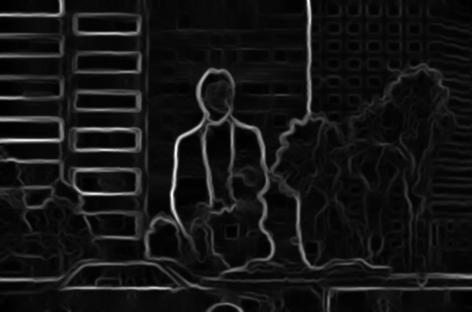
\includegraphics[width=2cm]{fig/119082[7-JOR]_crisp.jpg} \\
  AUC: 0.829 & 0.671 & 0.782 & 0.763 & 0.821 & 0.803 & 0.820 \\ 
  \hspace{-2mm}
  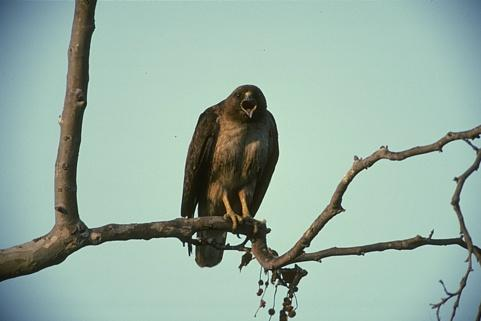
\includegraphics[width=2cm]{fig/42049_g.jpg} & \hspace{-4mm}
  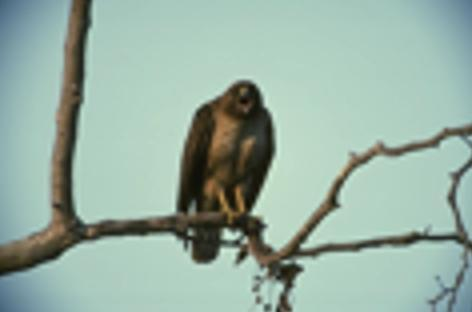
\includegraphics[width=2cm]{fig/42049[2-Bicubic]_g.jpg} & \hspace{-4mm}
  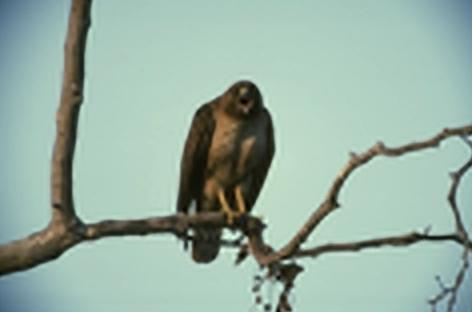
\includegraphics[width=2cm]{fig/42049[3-Zeyde]_g.jpg} & \hspace{-4mm}
  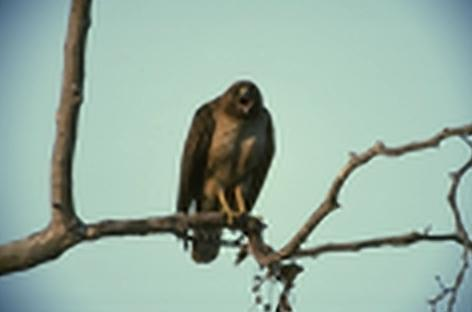
\includegraphics[width=2cm]{fig/42049[4-ANR]_g.jpg} & \hspace{-4mm}
  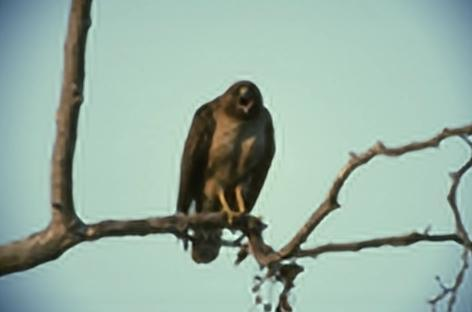
\includegraphics[width=2cm]{fig/42049[5-SRCNN]_g.jpg} & \hspace{-4mm}
  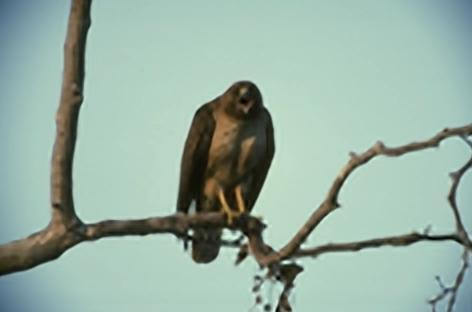
\includegraphics[width=2cm]{fig/42049[6-A+]_g.jpg} & \hspace{-4mm}
  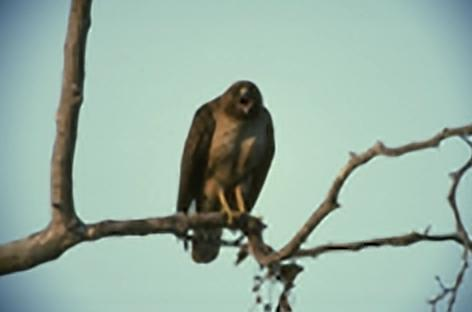
\includegraphics[width=2cm]{fig/42049[7-JOR]_g.jpg} \\
  PSNR & 26.94 & 28.29 & 28.06 & 29.05 & 29.17 & 28.93 \\    
  \hspace{-2mm}
  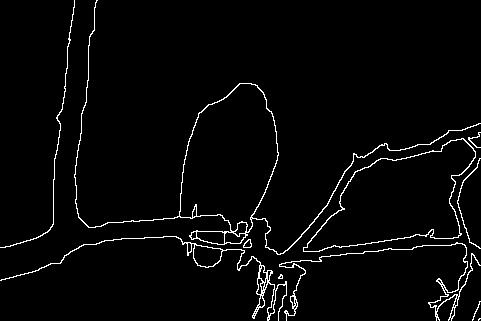
\includegraphics[width=2cm]{fig/42049_seg.jpg} & \hspace{-4mm}
  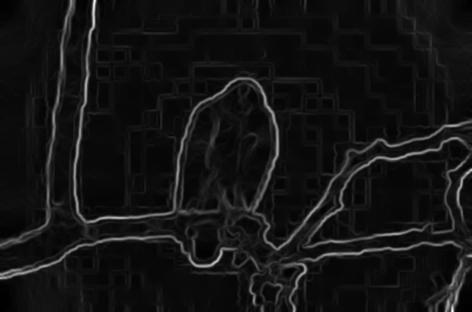
\includegraphics[width=2cm]{fig/42049[2-Bicubic]_crisp.jpg} & \hspace{-4mm}
  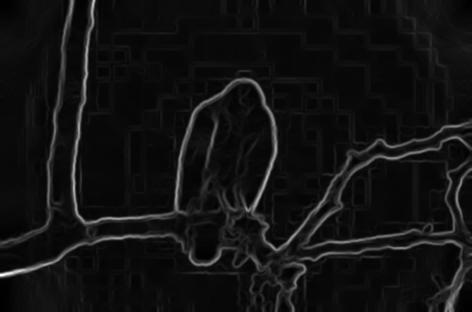
\includegraphics[width=2cm]{fig/42049[3-Zeyde]_crisp.jpg} & \hspace{-4mm}
  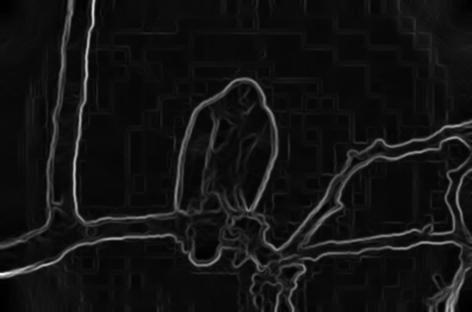
\includegraphics[width=2cm]{fig/42049[4-ANR]_crisp.jpg} & \hspace{-4mm}
  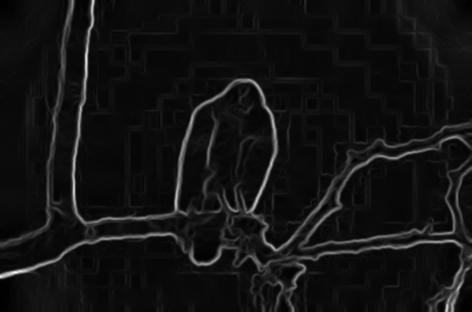
\includegraphics[width=2cm]{fig/42049[5-SRCNN]_crisp.jpg} & \hspace{-4mm}
  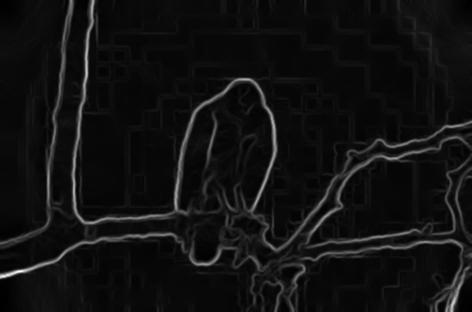
\includegraphics[width=2cm]{fig/42049[6-A+]_crisp.jpg} & \hspace{-4mm}
  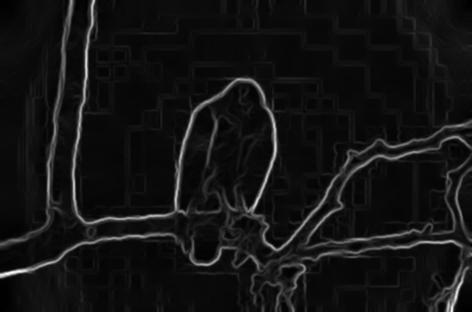
\includegraphics[width=2cm]{fig/42049[7-JOR]_crisp.jpg} \\
  AUC: 0.905 & 0.851 & 0.878 & 0.907 & 0.873 & 0.895 & 0.907 \\ 
  \hspace{-2mm}
  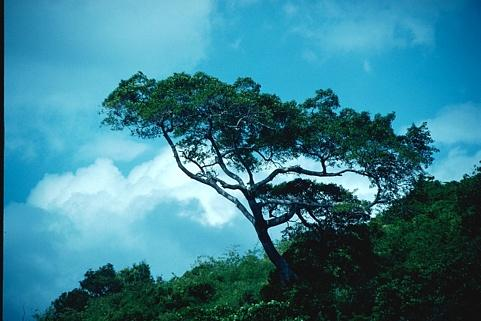
\includegraphics[width=2cm]{fig/147091_g.jpg} & \hspace{-4mm}
  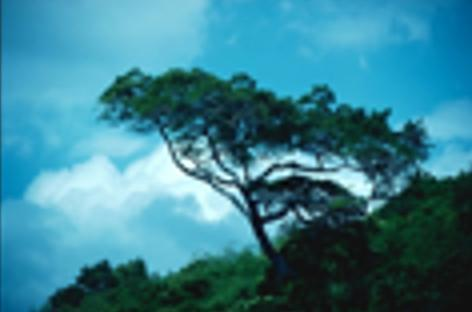
\includegraphics[width=2cm]{fig/147091[2-Bicubic]_g.jpg} & \hspace{-4mm}
  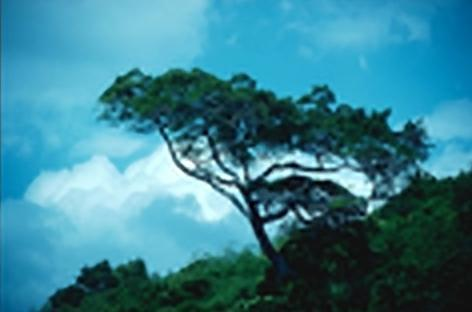
\includegraphics[width=2cm]{fig/147091[3-Zeyde]_g.jpg} & \hspace{-4mm}
  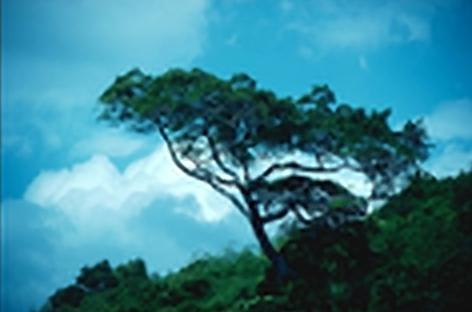
\includegraphics[width=2cm]{fig/147091[4-ANR]_g.jpg} & \hspace{-4mm}
  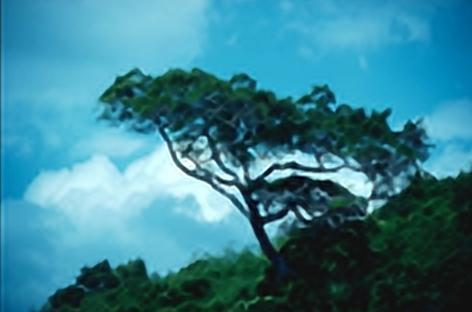
\includegraphics[width=2cm]{fig/147091[5-SRCNN]_g.jpg} & \hspace{-4mm}
  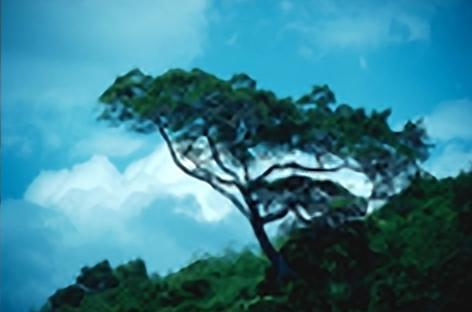
\includegraphics[width=2cm]{fig/147091[6-A+]_g.jpg} & \hspace{-4mm}
  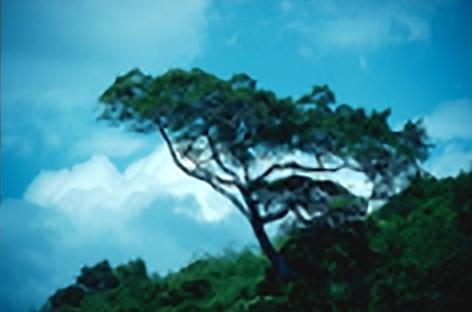
\includegraphics[width=2cm]{fig/147091[7-JOR]_g.jpg} \\
  PSNR & 24.41 & 24.93 & 24.95 & 25.13 & 25.13 & 25.11\\       
  \hspace{-2mm}
  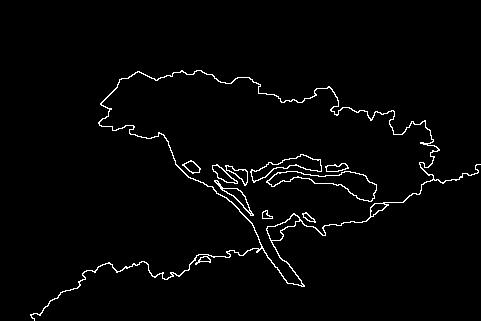
\includegraphics[width=2cm]{fig/147091_seg.jpg} & \hspace{-4mm}
  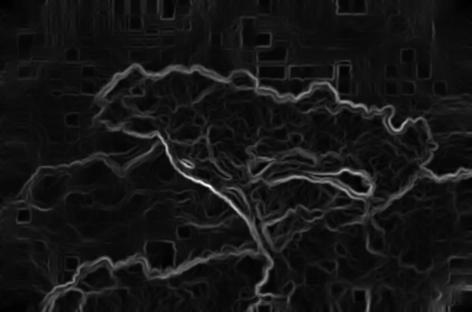
\includegraphics[width=2cm]{fig/147091[2-Bicubic]_crisp.jpg} & \hspace{-4mm}
  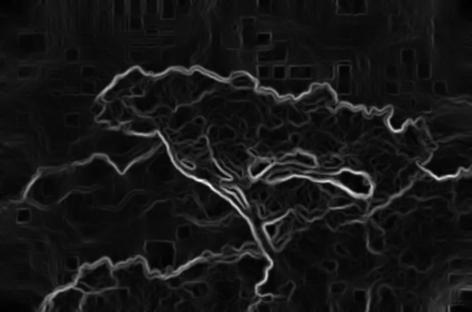
\includegraphics[width=2cm]{fig/147091[3-Zeyde]_crisp.jpg} & \hspace{-4mm}
  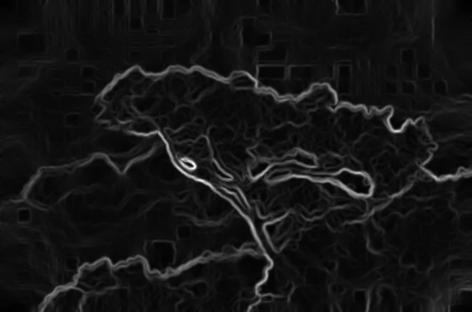
\includegraphics[width=2cm]{fig/147091[4-ANR]_crisp.jpg} & \hspace{-4mm}
  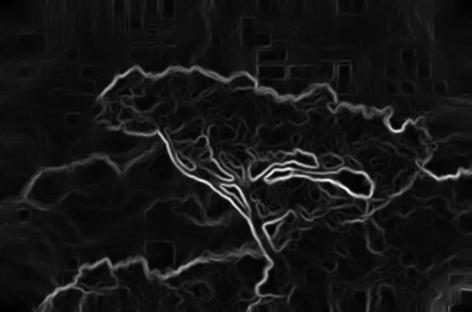
\includegraphics[width=2cm]{fig/147091[5-SRCNN]_crisp.jpg} & \hspace{-4mm}
  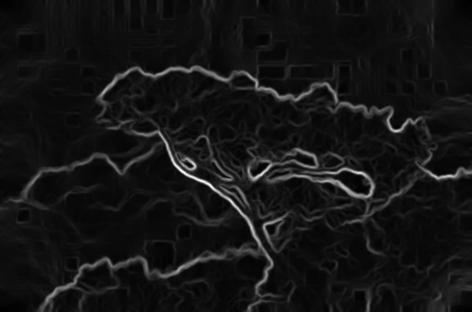
\includegraphics[width=2cm]{fig/147091[6-A+]_crisp.jpg} & \hspace{-4mm}
  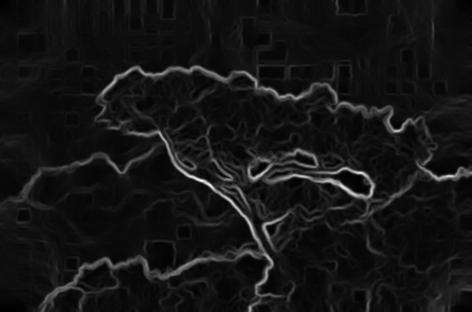
\includegraphics[width=2cm]{fig/147091[7-JOR]_crisp.jpg} \\
  AUC: 0.827 & 0.690 & 0.752 & 0.772 & 0.799 & 0.787 & 0.783 \\
    \hspace{-2mm}
  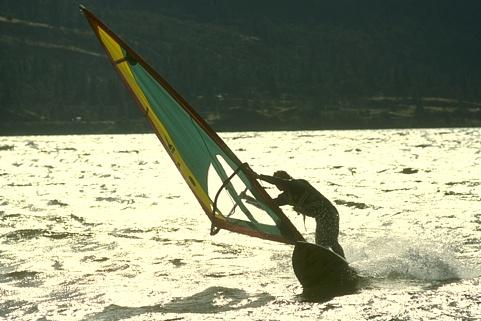
\includegraphics[width=2cm]{fig/62096_g.jpg} & \hspace{-4mm}
  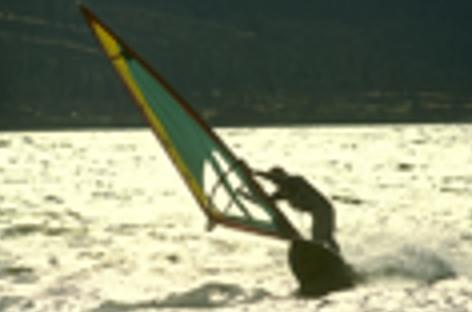
\includegraphics[width=2cm]{fig/62096[2-Bicubic]_g.jpg} & \hspace{-4mm}
  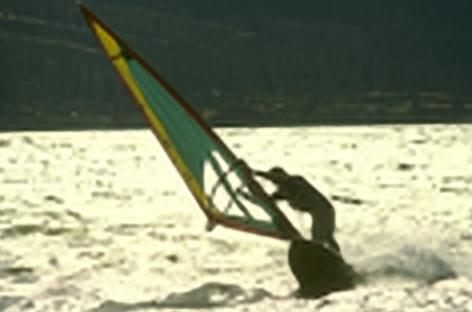
\includegraphics[width=2cm]{fig/62096[3-Zeyde]_g.jpg} & \hspace{-4mm}
  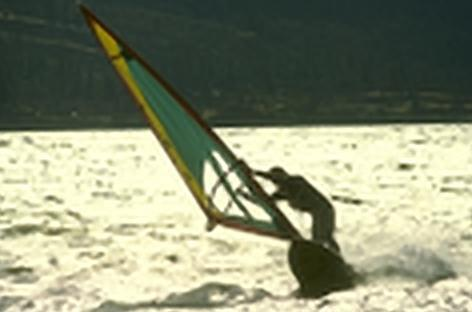
\includegraphics[width=2cm]{fig/62096[4-ANR]_g.jpg} & \hspace{-4mm}
  \includegraphics[width=2cm]{fig/62096[5-SRCNN]_g.jpg} & \hspace{-4mm}
  \includegraphics[width=2cm]{fig/62096[6-A+]_g.jpg} & \hspace{-4mm}
  \includegraphics[width=2cm]{fig/62096[7-JOR]_g.jpg} \\
  PSNR & 23.40 & 24.11 & 24.02 & 25.54 & 24.41 & 24.46 \\    
  \hspace{-2mm}
  \includegraphics[width=2cm]{fig/62096_seg.jpg} & \hspace{-4mm}
  \includegraphics[width=2cm]{fig/62096[2-Bicubic]_crisp.jpg} & \hspace{-4mm}
  \includegraphics[width=2cm]{fig/62096[3-Zeyde]_crisp.jpg} & \hspace{-4mm}
  \includegraphics[width=2cm]{fig/62096[4-ANR]_crisp.jpg} & \hspace{-4mm}
  \includegraphics[width=2cm]{fig/62096[5-SRCNN]_crisp.jpg} & \hspace{-4mm}
  \includegraphics[width=2cm]{fig/62096[6-A+]_crisp.jpg} & \hspace{-4mm}
  \includegraphics[width=2cm]{fig/62096[7-JOR]_crisp.jpg} \\
  AUC: 0.902 & 0.778 & 0.845 & 0.820 & 0.855 & 0.852 & 0.833 \\

\end{tabular*}
   \caption{Sampled super-resolved images with their PSNR values and corresponding detected boundary maps by CBD~\cite{isola2014crisp} with their AUC values. Zeyde et al. works similarly to ANR, and A+ and SRCNN works similarly to JOR, so only ANR and JOR are shown. }
\label{fig:ed_cbd}  
\end{figure*}

\subsection{Image Labeling}
\label{sec:il}



\begin{table} [tb]\small{   \centering
%\footnotesize
\centering
\caption{Average PSNR and labeling accuracy on MSRC-21 dataset, where APP indicates Average Precision over Pixels, and APC means Average Precision over Classes. The best performance is shown in \textbf{bold} and the second best is \underline{underlined}.}
\resizebox{0.5\textwidth}{!}
{
\begin{tabular}{|l|c|cccccc|c|c|c|}
\hline
%\multicolumn{2}{|c||}{Benchmark} &Bicubic&SF&Zeyde~\cite{Zeyde-CS-2012}&GR~\cite{Timofte-ICCV-2013}& ANR~\cite{Timofte-ICCV-2013}& NE+LS~\cite{Timofte-ICCV-2013}& NE+NNLS~\cite{Timofte-ICCV-2013}& NE+LLE~\cite{Timofte-ICCV-2013}& SRCNN~\cite{Dong-ECCV-2014}&\textbf{A+}~\cite{Timofte-ICCV-2013}\\
\multicolumn{2}{|c|}{MSRC-21} & Bicubic&Zeyde~\etal& ANR& SRCNN & A+ &JOR  & Original \\
\multicolumn{2}{|c|}{ } & &\cite{Zeyde-CS-2012}& \cite{Timofte-ICCV-2013}& \cite{Dong-ECCV-2014} & \cite{Timofte-ACCV-2014} &\cite{JOR:EG15} & \\
\hline\hline
              %& x2 & 33.66 & 35.63 & 35.13 & 35.83 & 35.66 & 35.43 & 35.77 & \textbf{36.34} & 36.25\\
\textbf{$\times$3} & PSNR & 25.29 & 26.02 & 26.00 & \underline{26.21} & \textbf{26.28} & \textbf{26.28} & --- \\
            & SSIM & 0.689 & 0.726 & 0.728 & \underline{0.733} & \textbf{0.737} & \textbf{0.737} & --- \\
            & IFC & 2.677 & 3.214 & 3.250 & 3.131 & \underline{3.390} & \textbf{3.396} & --- \\
            & NQM & 19.56 & 22.48 & 22.47 & 22.64 & \underline{23.10} & \textbf{23.16} & --- \\
            \hline
            & APP & 0.692 & 0.762 & 0.770 & 0.777 & \underline{0.780}  & \textbf{0.783} &0.844 \\
            & APC & 0.592 & 0.662 & 0.674 & 0.681 & \underline{0.684}  & \textbf{0.687} & 0.743 \\
\hline

\textbf{$\times$4} & PSNR & 24.04 & 24.65 & 24.63 & 24.77 & \textbf{24.88} & \underline{24.86} & --- \\
            & SSIM & 0.608 & 0.641 & 0.643 & 0.646 & \textbf{0.654} & \underline{0.652} & --- \\
            & IFC & 1.694 & 2.043 & 2.066 & 1.992 & \textbf{2.171} & \underline{2.155} & --- \\
            & NQM & 14.75 & 16.56 & 16.55 & 16.73 & \underline{17.10} & \textbf{17.12} & --- \\
            \hline
            & APP & 0.582 & 0.665 & 0.677 & 0.673 & \textbf{0.682} & \underline{0.674} & 0.844 \\
            & APC & 0.505 & 0.569 & 0.584 & \underline{0.588} & \textbf{0.591} & 0.586 & 0.749 \\
\hline
\end{tabular}
}
\label{tab:il}}
\end{table}


\begin{figure*} [tb]
\begin{tabular*}{0.5\textwidth}{cccc} 
 (a) Original & (b) Bicubic & (c) ANR & (d) JOR \\  
\hspace{-2mm}
\includegraphics[width=2cm]{fig/1_30_s_o_lmnn_5_img.jpg} & \hspace{-4mm}
\includegraphics[width=2cm]{fig/1_30_s_B_lmnn_5_img.jpg} & \hspace{-4mm}
\includegraphics[width=2cm]{fig/1_30_s_A_lmnn_5_img.jpg} & \hspace{-4mm}
\includegraphics[width=2cm]{fig/1_30_s_J_lmnn_5_img.jpg} \\
-- & PSNR / 26.24  & PSNR / 26.64  & PSNR / 26.72 \\    \hspace{-2mm}
\includegraphics[width=2cm]{fig/1_30_s_o_lmnn_5_label.jpg} & \hspace{-4mm}
\includegraphics[width=2cm]{fig/1_30_s_B_lmnn_5_label.jpg} &\hspace{-4mm}
\includegraphics[width=2cm]{fig/1_30_s_A_lmnn_5_label.jpg} &\hspace{-4mm}
\includegraphics[width=2cm]{fig/1_30_s_J_lmnn_5_label.jpg} \\
APP / 0.975 & APP / 0.902 & APP / 0.954 & APP / 0.957 \\

\hspace{-2mm}
\includegraphics[width=2cm]{fig/3_22_s_o_lmnn_5_img.jpg} &\hspace{-4mm}
\includegraphics[width=2cm]{fig/3_22_s_B_lmnn_5_img.jpg} &\hspace{-4mm}
\includegraphics[width=2cm]{fig/3_22_s_A_lmnn_5_img.jpg} &\hspace{-4mm}
\includegraphics[width=2cm]{fig/3_22_s_J_lmnn_5_img.jpg} \\
 --- & PSNR / 24.04  & PSNR / 24.53  & PSNR / 24.76 \\   \hspace{-2mm}
\includegraphics[width=2cm]{fig/3_22_s_o_lmnn_5_label.jpg} &\hspace{-4mm}
\includegraphics[width=2cm]{fig/3_22_s_B_lmnn_5_label.jpg} &\hspace{-4mm}
\includegraphics[width=2cm]{fig/3_22_s_A_lmnn_5_label.jpg} &\hspace{-4mm}
\includegraphics[width=2cm]{fig/3_22_s_J_lmnn_5_label.jpg} \\
APP / 0.937 & APP / 0.639 & APP / 0.888 & APP / 0.909 \\
\end{tabular*}
   \caption{Examples for image labeling: super-resolved images with their PSNR values and the corresponding labeling results with their average precision over pixels (APP) are shown. Zeyde et al. works similarly to ANR, and A+ and SRCNN works similarly to JOR, so only  the results of ANR and JOR are shown.}
\label{fig:example:il}
\end{figure*}


%In this section, we evaluate ISR methods on the task of image labeling. 
%Image labeling aims to assign a semantic label to each pixel of an image. There is a very rich literature addressing semantic image labeling. Reviewing all of them is out the scope of this paper. We follow the footsteps of most previous work on image labeling and choose the well-known dataset MSRC-21 for the evaluation. MSRC-21 consists of 591 images of 21 semantic categories, , such as \emph{tree}, \emph{road}, and \emph{car}. For the labeling method, we employ the very recent one~\cite{superpixel:eccv14}, which presents a fast nearest neighbor approach via building a graph over superpixels over annotated set of training images and test images with learned weights for the linking edges to transfer labels from training images to test image.  The method shows comparable reautls to the state-of-the-art. The model is trained with original training images. For the implementation, we use the authors' code directly with the default settings.

In this section, we consider the task of image labeling. Image labeling, or semantic segmentation, aims to assign a semantic label to each pixel of an image, such as \emph{tree}, \emph{road}, and \emph{car}. It is a very popular high-level vision task with a large number of methods proposed~\cite{texton-forests, Gould:decomposing:ICCV09, dai:eccv12a, superpixel:eccv14}.  We follow the footsteps of most previous works on image labeling and choose the standard MSRC-21~\cite{Shotton:2006:ECCV} dataset for the evaluation. MSRC-21 consists of 591 images of 21 semantic categories. For the labeling method, we employ the very recent approach~\cite{superpixel:eccv14}, which presents a fast approximate nearest neighbor algorithm for image labeling. They build a super-pixel graph from annotated set of training images. At test time, they transfer labels from the training images to the test image via matching super-pixels in the graph. The distance between super-pixels in the feature space is approximated by edge distance in the super-pixel graph where the edge weights are learned from the training set. This method shows comparable results to the state-of-the-art methods. For the implementation, we use the authors' code directly with the default settings. 


In order to evaluate the ISR methods for image labeling, we train the method~\cite{superpixel:eccv14} with the original training images and test the trained model on seven versions of the testing images, created by downsampling the original images and then upsampling them by the ISR methods to the resolution of the original images. Again, the performance is tested for scaling factor x3 and x4. 
Table~\ref{tab:il} lists the results of all ISR methods, where the average precision over pixels (APP) and the average precision over classes (APC) are reported, along with the average PSNR values. As we can see from the table, all the five ISR methods yield significantly  better results than the Bicubic Interpolation. Put it into another words, these learning-based super-resolution systems, in addition to improving visual quality of LR images, do facilitate image semantic labeling tasks and improve the performance substantially when the resolution of the testing images are lower than that of the training images. The results suggest that it is worth investigation to integrate ISR methods into real image labeling systems if the resolutions of training and testing images are distinctive. This is highly probably the case for real labeling systems where training images on the server side are from expensive sensors and testing images are from cheap sensors such as cameras of mobile phones. Another observation from the table is that the standard perceptual evaluation criterion PSNR correlates quite well with the usefulness of ISR methods for image labeling. This implies that good visual quality also facilitates computer systems for recognition. This can ascribed to the task of image labeling are defined by human and computer are trained to complete a human vision task which is of course very relevant to perceptual quality of images. Also, ISR methods are more useful when the scaling factor is larger, which means they are mostly needed when the input images are of very low-resolution.  The observations are consistent with that of BD described in Sec.~\ref{sec:ed}. 

In Fig.~\ref{fig:example:il}, we show two image examples, with the super-resolution results and their corresponding image labeling results. From the figure, it is evident that ISR methods improve the quality of the labeling results. For instance, in the second example, results of Bicubic Interpolation labeled a large area of the building to sky, which is probably due to the detailed textures on the wall of the building are missing in the interpolated image, but is recovered (to some extend) by the example-based ISR methods, leading to better labeling results.   



\subsection{Digit Recognition}
\label{sec:dr}
In this section, we test the usefulness of ISR methods for the task of digit recognition where the training images and the test image are both of low-resolution.  
We use the Street View House Numbers (SVHN)~\cite{37648} dataset which contains more than 100,000 images of house numbers obtained from Google Street View. Each image presents a single digit at its center and has the same size of 32$\times$32 pixels. 
We select 26,032 and 10,000 images from the dataset as our training and test set. 
In order to evaluate the usefulness of ISR methods for digit recognition, we here downsample all the images by factor x4 and upsample the downsampled images to the resolution of the original images by the ISR methods.
As the SVHN dataset merely presents numbers from 0 to 9, it is highly specific and quite different from the training dataset  from~\cite{Yang-TIP-2010} that is used to train our ISR methods. Therefore, we introduce a new ISR method by training A+ method with the unused images from the SVHN dataset, to study the generality of ISR methods. After adding the re-trained A+ method, we now have six datasets of super-resolved results, one set of data from Bicubic Interpolatin and one dataset of original images. 
% By doing so, the training and testing images are the super-resolved results from each of the ISR methods. 
We use the kNN classifier with $k=5$ for each of the eight image sets with HOG feature~\cite{Dalal_HoG} as input. 


% We then make an adjustment to the original datasets as we cut off a border of 4 pixels wide from all images. Such adjustment aims to get rid of meaningless backgrounds and emphasize the digits. After that, we downscale all cropped images by four and operate the upscaling with all six ISR methods to create six pairs of super-resolved training and test sets. 

The classification performance is listed in Table~\ref{tab:dr}. As Table~\ref{tab:dr} demonstrates, that ISR methods does improve the performance of digit recognition over simple interpolation, and that the PSNR values correlate well with the usefulness of ISR methods for digit recognition. The reason of the improvement is because HOG feature was designed for images of normal resolution, so by applying ISR methods to LR input images, HOG can be extracted from images of more suitable resolution.   
However, we find that with the standard, general training dataset~\cite{Yang-TIP-2010}, Zeyde et al. and ANR perform better than SRCNN, A+ and JOR, which is different the results on other datasets of general images. 
This observation suggests that Zeyde et al. and ANR are more generally applied than the other three state-of-the-art methods. The problem can be solved by retraining the model. We retrained the A+ method, and as expected the performance is improved significantly. In Fig.~\ref{fig:dr}, we show two examples of the digits, along with their super-resolved results and the PSNR values. From the figure, it is clear to see the artifacts generated by the generally trained ISR methods, especially by the SRCNN method, which comes with the most complicated model and seems to have the worst generality. The introduced artifacts confuse the classifiers.  



% It can be noticed that Zeyde \etal and ANR methods both perform well in this digit recognition task despite of their mediocre score in previous tasks. On the other hand, the SRCNN method suffers an astonishing drop-off and is outscored by naive Bicubic interpolation. It can also be noticed that the re-trained A+ method achieves the highest PSNR and classification accuracy at the same time. This result suggests that the learning process affects the performance of ISR methods. More specifically, an ISR method tends to perform better if it is trained by a dataset that is relative to the task. It helps to explain SRCNN's drop-off as the SVHN dataset contains much smaller and quite different images compared to the standard dataset that SRCNN is initially trained on. In that case, the SRCNN method may not be robust since it is based on deep convolutional neural network. 




\begin{figure}
\resizebox{0.5\textwidth}{!}{
\begin{tabular}{cccccccc}
 Bicubic & Zeyde & ANR & SRCNN & A+ & JOR & A+[R] & Original  \\  
  \includegraphics[width = 0.05\textwidth]{./fig/digit_0_bicubic.jpg} & 
  \includegraphics[width = 0.05\textwidth]{./fig/digit_0_zeyde.jpg} & 
  \includegraphics[width = 0.05\textwidth]{./fig/digit_0_anr.jpg} & 
  \includegraphics[width = 0.05\textwidth]{./fig/digit_0_srcnn.jpg} & 
  \includegraphics[width = 0.05\textwidth]{./fig/digit_0_aplus.jpg} & 
  \includegraphics[width = 0.05\textwidth]{./fig/digit_0_jor.jpg} & 
  \includegraphics[width = 0.05\textwidth]{./fig/digit_0_aplus_r.jpg} &
    \includegraphics[width = 0.05\textwidth]{./fig/digit_0_original.jpg}  \\
   23.84 & 28.96 & 28.13 & 23.89 & 27.43 & 23.89 & 31.32 & --- \\
  \includegraphics[width = 0.05\textwidth]{./fig/digit_6_bicubic.jpg} & 
  \includegraphics[width = 0.05\textwidth]{./fig/digit_6_zeyde.jpg} & 
  \includegraphics[width = 0.05\textwidth]{./fig/digit_6_anr.jpg} & 
  \includegraphics[width = 0.05\textwidth]{./fig/digit_6_srcnn.jpg} & 
  \includegraphics[width = 0.05\textwidth]{./fig/digit_6_aplus.jpg} & 
  \includegraphics[width = 0.05\textwidth]{./fig/digit_6_jor.jpg} & 
  \includegraphics[width = 0.05\textwidth]{./fig/digit_6_aplus_r.jpg} &
    \includegraphics[width = 0.05\textwidth]{./fig/digit_6_original.jpg} \\
  27.29 & 30.51 & 30.37 & 27.02 & 30.41 & 30.51 & 34.38 & --- \\
\end{tabular}
}
   \caption{Super-resolved results of two digits.}
\label{fig:dr}
\end{figure}


\begin{table} [tb] 
\small{ \centering
\resizebox{0.5\textwidth}{!}{
\begin{tabular}{|l|c|cccccc|c|c|c|} 
  \hline
  \multicolumn{2}{|c|}{SVHN}  & Bicubic & Zeyde~\etal & ANR & SRCNN & A+ & JOR & A+[R] & Original \\
  \multicolumn{2}{|c|}{ }  & & \cite{Zeyde-CS-2012} & \cite{Timofte-ICCV-2013} & \cite{Dong-ECCV-2014} & \cite{Timofte-ACCV-2014} & \cite{JOR:EG15} & & \\
  \hline
 $\times$3 & PSNR & 32.13 & 34.18 & \underline{34.52} & 25.33 & 33.63 & 33.68 & \textbf{35.84} & --- \\
  & SSIM & 0.907 & 0.943 & \underline{0.946} & 0.889 & 0.944 & \underline{0.946} & \textbf{0.957} & --- \\
  & IFC & 2.060 & 2.341 & \underline{2.429} & 1.703 & 2.402 & 2.355 & \textbf{2.694} & --- \\
  & NQM & 10.62 & 12.88 & \underline{13.20} & 9.65 & 12.38 & 12.43 & \textbf{14.36} & --- \\
  \hline
  & Accuracy & 0.734 & 0.745 & 0.746 & 0.716 & \underline{0.749} & 0.746 & \textbf{0.752} & 0.776  \\
  \hline
  $\times$4 & PSNR & 27.82 & 29.39 & \underline{29.49} & 26.37 & 29.23 & 29.23 & \textbf{30.47} & --- \\
  & SSIM & 0.776 & 0.835 & 0.840 & 0.792 & 0.840 & \underline{0.842} & \textbf{0.870} & --- \\
  & IFC & 1.268 & 1.357 & 1.372 & 1.144 & \underline{1.373} & 1.342 & \textbf{1.578} & --- \\
  & NQM & 6.513 & 8.096 & \underline{8.208} & 6.848 & 7.939 & 7.392 & \textbf{9.128} & --- \\
  \hline
  & Accuracy & 0.648 & 0.660 & \underline{0.664} & 0.641 & 0.656 & 0.654 & \textbf{0.680} & 0.776  \\
  \hline
  
\end{tabular}
}}
  \caption{Average PSNR values and accuracies of digit recognition on the SVHN dataset. The kNN classifier is trained and applied on HOG features of each pair of super-resolved training and test sets. A+[R] is the retrained A+. The best performance is shown in \textbf{bold} and the second best is \underline{underlined}.}
\label{tab:dr}
\end{table}

\subsection{Face Detection}
\label{sec:fr}

In this section, we investigate the usefulness of ISR methods for face detection. 
Face detection is widely used in security cameras and home surveillance systems, which has to deal with low-resolution inputs lots of time. 
It has proven by many works~\cite{face:SRTIP, face:SR08} that face super-resolution is helpful for the recognition. We in this section evaluate the usefulness of general ISR methods for face detection. 

% Therefore, a well performed ISR method is heavily needed to improve the quality of upscaled images and consequently boost the accuracy of face recognition systems. Inspired by the conclusions of previous tasks, we hope to establish a link between PSNR value of super-resolved images and face recognition accuracies as well.


The Face Detection Data Set and Benchmark (FDDB)~\cite{fddbTech}  is used, which contains 2845 facial images with 5171 human-annotated faces. The super-resolved datasets are generated again by downsampling the images by $\times$4 and then upscaling them to the resolution of the original images. We then apply the well-known Viola-Jones algorithm~\cite{viola2001rapid} on each of the super-resolved datasets, the result of Bicubic Interpolation, and the original dataset to obtain the bounding boxes of detected faces. 
We use the default Matlab implementation of Viola-Jones detector, a pre-trained detector with images of `normal' resolution, to test its performance on the seven versions of the test images.  To evaluate accuracies of detected faces, we use both continuous and discrete true positive percentages as described in ~\cite{fddbTech}. 

% Let $d_i$ and $a_i$ denote the $i^{th}$ detection and corresponding annotation. The score $y_i$ for this detection is defined as below:
% $$Discrete \ Score: y_i = \delta_{S(d_i,a_i)>THR}$$
% $$Continuous \ Score: y_i = S(d_i,a_i)$$
% Function \emph{S} represents the degree of match and is employed as the ratio of intersected areas to joined areas while parameter THR sets a threshold on the matches.
% $$S(d_i,a_j)=\frac{area(d_i) \cap area(a_j)}{area(d_i) \cup area(a_j)}\qquad$$


Table~\ref{tab:fr} demonstrates continuous and discrete true positive scores with parameter \emph{THR} (matching threshold for positives) set to 0.5. As it turns out, ISR methods are also helpful for the task of face detection, relative to Bicubic Interpolation. The relationship between PSNR values and two TP scores is consistent with the conclusions in previous tasks: 
PSNR generally correlates well with the usefulness of ISR methods for face detection, but it is not accurate for the prediction. 
In particular,  A+ and JOR achieve the best performance. Zeyde et al. and ANR have very similar PSNR values while yielding quite different discrete TP values for face detection.   
We also show the performance of face detection with different values of THR in Fig.~\ref{fig:fr}, from which it can be seen that the conclusion for THR=0.5 holds for other values of  THR as well. 


% All in all, the conclusion is still ISR methods should be considered as a preprocessing step for face detection if the resolution of faces are low, and ISR methods needs to be integrated into the real detection systems for a precise evaluation of their usefulness for face detection. 




\begin{table} [tb]
\small{  \centering
\resizebox{0.5\textwidth}{!}{
\begin{tabular}{|l|c|cccccc|c|c|c|}
\hline
\multicolumn{2}{|c|}{FDDB} & Bicubic & Zeyde~\etal & ANR & SRCNN & A+ & JOR & Original \\
\multicolumn{2}{|c|}{THR = 0.5} & &\cite{Zeyde-CS-2012}& \cite{Timofte-ICCV-2013}& \cite{Dong-ECCV-2014} & \cite{Timofte-ACCV-2014} &\cite{JOR:EG15} & \\
\hline\hline
\textbf{$\times$3} & PSNR & 29.77 & 31.38 & 31.35 & \underline{31.57} & 31.24 & \textbf{31.99} & --- \\
                   & SSIM & 0.883 & 0.906 & \underline{0.907} & 0.897 & 0.905 & \textbf{0.914} & --- \\
                   & IFC & 3.598 & 4.395 & 4.494 & 4.079 & \underline{4.496} & \textbf{4.707} & --- \\
                   & NQM & 31.49 & 37.58 & 37.75 & 34.51 & \underline{37.93} & \textbf{38.48} & --- \\
                   \hline
                   & \emph{disc.} TP(\%) & 72.15 & 72.64 & \underline{72.79} & 72.71 & 72.60 & \textbf{72.93} & 73.04 \\
                   & \emph{cont.} TP(\%) & 47.15 & 47.47 & \underline{47.56} & 47.53 & 47.46 & \textbf{47.64} & 47.72 \\
\hline

\textbf{$\times$4} & PSNR & 27.76 & 29.16 & 29.09 & 28.88 & \textbf{29.76} & \underline{29.68} & --- \\
                   & SSIM & 0.832 & 0.858 & 0.858 & 0.832 & \textbf{0.870} & \underline{0.869} & --- \\
                   & IFC & 2.467 & 2.959 & 2.993 & 2.624 & \textbf{3.185} & \underline{3.138} & --- \\
                   & NQM & 24.79 & 29.91 & 30.02 & 26.13 & \textbf{31.16} & \underline{31.03} & --- \\
                   \hline
                   & \emph{disc.} TP(\%) & 70.82 & 71.38 & 71.46 & 71.46 & \textbf{71.55} & \underline{71.48} & 73.04 \\
                   & \emph{cont.} TP(\%) & 46.29 & 46.65 & 46.65 & 46.70 & \textbf{46.78} & \underline{46.73} & 47.72 \\
\hline
\end{tabular}
}
\caption{Average PSNR value together with continuous and discrete true positive scores on the FDDB dataset. Both kinds of TP scores are obtained using Viola-Jones face detector in Matlab and the parameter \emph{THR} is fixed to 0.5. The best performance is shown in \textbf{bold} and the second best is \underline{underlined}.}
\label{tab:fr} }
\end{table}

\begin{figure}
  \centering
  \includegraphics[width = 0.5\textwidth]%
    {fig/fr_vj_cont_tp_thr.eps}% picture filename
  \caption{Continuous true positive percentage of face detection on all the super-resolved datasets and the original dataset with different matching thresholds for positives (\emph{THR}), intersection over union. All results are drawn relative to the results of Bicubic Interpolation for visual clarity.}
\label{fig:fr}
\end{figure}


\section{Conclusion}
\label{sec:conclusion}
We have evaluated the usefulness of image super-resolution (ISR) for a variety of different vision tasks.  Five ISR methods have been employed and evaluated on four popular vision tasks. Three conclusions can be drawn from the experiments: 1) ISR methods are helpful in general for other vision tasks when the resolution of input images are low; 2) all example-based ISR methods perform substantially better than simple Bicubic Interpolation, and JOR and A+ are most useful among alternatives for other vision tasks; 3) standard perceptual criterion PSNR correlates generally well with the usefulness of ISR methods for other vision tasks, but it is not accurate as a direct measurement. We hope this work will be an inspiration for the community to 1) integrate ISR methods into other practical vision systems when the input images are of low-resolution; and 2) to evaluate ISR methods in real vision tasks, in addition to merely inspecting the visual quality. 

{\small
\bibliographystyle{ieee}
\bibliography{egbib}
}


\end{document}
